This section describes our approach to specifying and updating robot missions taking place in open worlds. 
Our presentation takes the form of requirements on a specification language $\Lambda$, such that mission specifications $\mathcal{M}(AP) \in \Lambda$, parsed by $\mathcal{P}_{\Lambda}$ satisfy Eq. \eqref{Eq:newSpec}. 

First, we leverage the expressive power of open-world abstraction to specify high-level behaviors without referring to individual propositions $\pi \in AP_k$ exclusively. 
Then, we show that the addition of propositions to a mission specification $\mathcal{M}_k = \mathcal{M}(AP_k)$ has to follow certain rules in order to maintain the correspondence $\mathcal{C}: AP \rightarrow AP^{n}$ between propositions. Finally, we provide a mechanism that allows the user to explicitly specify when the updated specification $\mathcal{M}_{k+1} \mathcal{M}(AP_{k+1})$, and consequently the GR(1) formula $\varphi [k+1] = \mathcal{P}_{\Lambda} (\mathcal{M}_{k+1}, AP_{k+1})$, should be translated into a revised robot controller.

\subsection{Defining Tasks over Open Worlds}

The first requirement on missions $\mathcal{M}(AP) \in \Lambda$ is the definition of groups of propositions $G_i$ and the definition of correspondence between propositions or groups of propositions. Then, tasks that refer to individual propositions $\pi \in G_i$ can be replaced by tasks over $G_i$ and $G_j \in \mathcal{C}(G_i), \; j \not = i$.

We revisit Example \ref{Ex:mailbot1} and make use of the open world abstractions. For illustrative purposes, we use Structured English \cite{JFRKGICRA12} as the specification language $\Lambda$.

\begin{myExample}\label{Ex:mailbot2} Autonomous Mailbot (revisited)\\
\texttt{Group Letters is letter1, letter2} \# $G_1$ \\
\texttt{Group Offices is office1, office2} \# $G_2$ \\
\texttt{Letters correspond to Offices} \# $G_2 \in \mathcal{C}(G_1)$\\
\texttt{if you are sensing any Letter then do PickUp and go to corresponding Office}\\ 
where $G_1 = \texttt{Letters}$ and $G_2 = \texttt{Offices}$ are groups of environment and robot (region) propositions, respectively.
\end{myExample}
Notice how the sentence describing the task (lines 4-5) does not refer to any particular letters (\texttt{letter1}, \texttt{letter2}) or offices (\texttt{office1}, \texttt{office2}). 
In fact, even if the groups were empty, i.e., $G_1, G_2 = \left\{ \right\}$, the user would still be able to specify the mission above.
Moreover, the reason we used the notation $G_2 \in \mathcal{C}(G_1)$, rather than $G_2 = \mathcal{C}(G_1)$, is that $G_1$ could potential correspond to more groups, e.g. $\mathcal{C}(G_1) = \left\{ G_2, G_3, \ldots\right\}$

If a letter corresponding to a new recipient is sensed by a ``new letter sensor", $d_{m} = \texttt{newLetter} \in \mathcal{D}$, a new proposition, $\pi_{mt} = $\texttt{letter3}, would be added to $AP_t$. 
There are two requirements for the mission in Example \ref{Ex:mailbot2} to reflect the addition of the new proposition. 
First, $\pi_{mt}$ has to be added to $G_1$, not just the set of all propositions $AP_t$. 
Second, an office proposition, $\pi_{mt}^{(2)} = \texttt{office3}$, has to be created, if necessary, and added to $G_2$, in order to reestablish correspondence, i.e., $G_2 \in \mathcal{C}(G_1)$, where now $G_{1} = G_1 \cup \left\{ \pi_{mt} \right\}$, $G_{2} = G_2 \cup \{ \pi_{mt}^{(2)} \}$. 
Then, we would have $\pi_{mt}^{(2)} \in \mathcal{C}(\pi_{mt})$. 
The two requirements are generalized in Problem \ref{Prob:correspondence}, a subproblem of Problem \ref{Prob:newSpec}:

\begin{myProblem}\label{Prob:correspondence}
	\textbf{(New Propositions and Correspondence):} Given a mission specification $\mathcal{M}_k$, and a new proposition $\pi_{mt} = D(m, t)$, define a mechanism for (i) adding $\pi_{mt}$ to a group of propositions $G_m$ in $\mathcal{M}_k$, and (ii) creating additional propositions, if necessary, and adding them to the corresponding groups $C(G_m)$.
\end{myProblem}

\subsection{Rewriting the Specification} % Re-synthesis (not local yet)

To address Problem \ref{Prob:correspondence}, we introduce another element to the specification language $\Lambda$, the ``add to Group" operator.

\begin{myDefinition}\label{Def:addto}
	\textbf{(add to Group):} When used in a sentence of $\mathcal{M} \in \Lambda$, the \emph{add to Group} operator takes the new proposition $\pi_{mt} = D(m,t)$, by reading the sensor preceding the operator, and adds it to its argument, a group of propositions $G_m$. 
	Furthermore, it creates additional propositions $\mathcal{C}(\pi_{mt})$, and adds them to the corresponding groups $\mathcal{C}(G_m)$. 
	
	More concisely:
	\begin{equation}
	\begin{split}
		\X d_m \Leftrightarrow &((G_m = G_m \cup \left\{ \pi_{mt} \right\}) \\
		\bigwedge_{G_i \in \mathcal{C}(G_m)} &(G_i = G_i \cup \left\{ \mathcal{C}(\pi_{mt}) \right\}))
	\end{split}
	\end{equation}
\end{myDefinition}
In Structured English, it would be used as follows: \texttt{if you are sensing somethingNew then add to GroupName}, where \texttt{somethingNew} $\in \mathcal{D}$. The new propositions are named either by a predefined naming scheme, by prompting the human user, or using information from the low-level sensor abstracted by $d_m \in \mathcal{D}$.

Since we are now adding propositions besides those added by the detection sensors $d_m \in \mathcal{D}$, as a direct result of the world being open, we have to restate Definition \ref{Def:openworld} as follows:

\begin{myDefinition}\label{Def:openworld2}	
	\textbf{(Expanding Open World Model -- revisited):} Our model $\W = \left\{ AP_0, AP_1, \ldots, AP_k \right\}$ is now updated such that the propositions added in order to maintain correspondence are also added to the set of atomic propositions. That is, 
	\begin{equation}\label{Eq:updateAP2}
		AP_{t+1} = AP_t \bigcup_{m=1}^{M}D(m, t) \bigcup_{m=1}^{M}\mathcal{C}(D(m, t)),
	\end{equation}
	replaces Eq. \eqref{Eq:updateAP}. Eq. \eqref{Eq:updateW} remains the same.
\end{myDefinition}

\begin{myAssumption}
	The grounding \cite{Grounding2013} of new propositions 
%	$\left\{ \pi_{mt}, \mathcal{C}(\pi_{mt}) \right\}$ 
$\pi \in AP_{k+1} \backslash AP_k$ to the robot's physical world is obtained either from the robot's low-level sensors, which propositions $d \in \mathcal{D}$ abstract, or by prompting the human user (Section \ref{simulation}).
Some auxiliary propositions, such as robot memory propositions, do not require grounding to the physical world.
%	The correspondence, i,e., the relationship of new elements of the open world to the robot's mission, is provided either by the robot's low-level sensors, or by prompting the human user. That is, for a proposition $\pi_{mk} = A(m, k)$, added to a group of propositions, the semantics of additional propositions $C(\pi_{mk})$ can be inferred.
	% Rephrase when Problem 2 is stated. Remember, you can use Groups now!
\end{myAssumption}

For instance, in Example \ref{Ex:mailbot2}, a new letter would result in new propositions, e.g. \texttt{letterNew} and \texttt{officeNew}. The sensor proposition \texttt{letterNew} would be grounded to the recipient's name on the letter. The information for grounding \texttt{officeNew} to a location on the robot's workspace can be inferred from the letter itself (address field), which the robot can look up in a digital map. If the new office is not part of the current map, the robot could prompt the user for its location, and then add it to its discrete abstraction of the workspace.

\subsection{Updating the Controller}

All the specification rewriting described so far has resulted in mission specification $\mathcal{M}_{k+1}$ that can be parsed to an LTL specification $\varphi [k+1]$, according to Eq. \eqref{Eq:newSpec}. However, for the updates to be reflected in the robot's controller, $\varphi [k+1]$ has to be passed to the synthesis algorithm in order to extract a new winning strategy. This process is dubbed ``re-synthesis" \cite{BingxinRSS2012}. We associate a robot proposition, e.g. \texttt{resynthesis}, with it. For example, in the setting of Example \ref{Ex:mailbot2}, and using Structured English, we could say:
\texttt{if you are sensing newLetter then add to Letters and do resynthesis}. 

Notice that the user chooses when re-synthesis will take place. Given the task above, the robot would update its strategy immediately after detecting a letter for a new recipient. In a search and rescue setting, it would make more sense for the robot to finish executing other actions before re-synthesizing.

\begin{myExample}\label{Ex:SnS} Search and Rescue Specification (partial)\\
	\texttt{Group Regions is \ldots}\\
	\texttt{visit each Region if and only if you are not activating rescueSurvivor}\\
	\texttt{if you are sensing newRegion then add to Regions and do needToResynthesize}\\
	\texttt{do resynthesis if and only if you are not activating rescueSurvivor and you are activating needToResynthesize}\\
	where \texttt{needToResynthesize} is a robot memory proposition that enables the robot to remember it detected a new region and that is has to re-synthesize eventually.
\end{myExample}

The definition of the \emph{add to Group} operator and \emph{resynthesis} conclude the augmentation of the specification language $\Lambda$. Our approach is graphically summarized in Fig. \ref{Fig:approach}, where  the part of $\mathcal{M}_{k+1}$ denoted as \texttt{Tasks} is immutable throughout the rewriting and re-synthesis processes.

\begin{figure}[h]
	\centering
	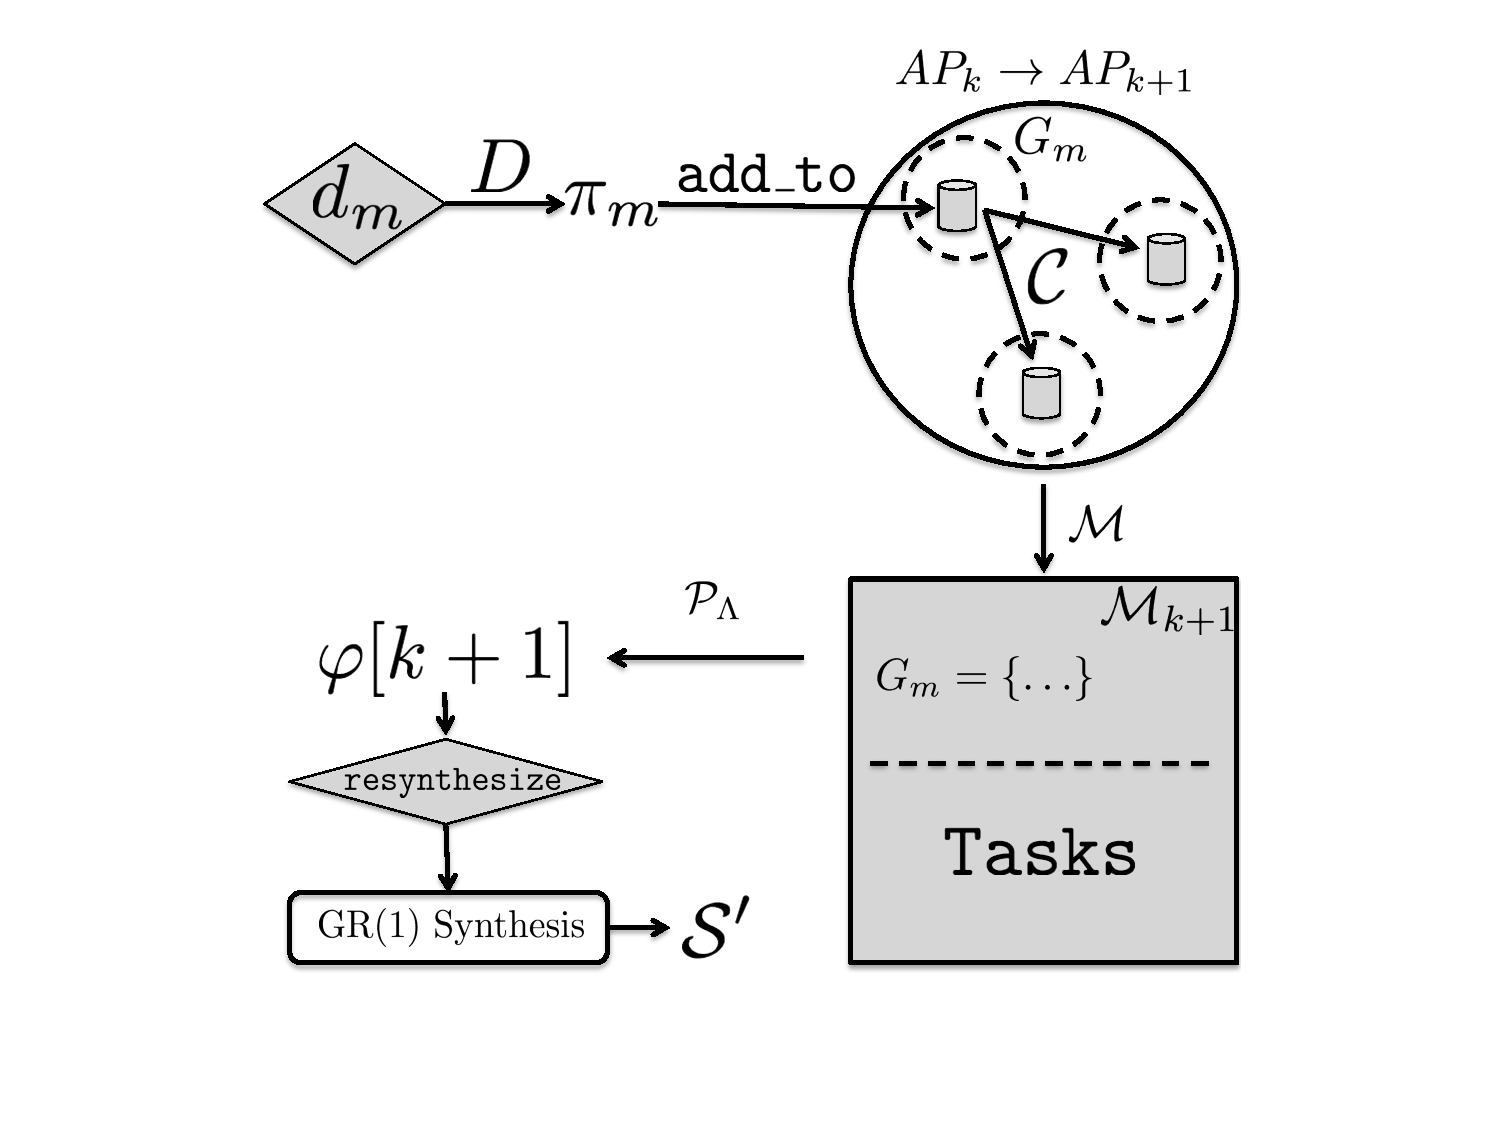
\includegraphics[width=0.9\columnwidth, clip]{./img/approach.pdf}
	\caption{\ldots} % TODO: Write stuff here
	\label{Fig:approach}
\end{figure}
% END